\begin{verbatim}


 [n, p, V, Fn, Fp, Jn, Jp, it, res] = secs1d_dd_newton (x, D, Vin, nin, 
                                                        pin, l2, er, un, 
                                                        up, theta, tn, tp, 
                                                        Cn, Cp, toll, maxit)

 Solve the scaled stationary bipolar DD equation system using Newton's method

     input: 
       x                spatial grid
       D                doping profile
       pin              initial guess for hole concentration
       nin              initial guess for electron concentration
       Vin              initial guess for electrostatic potential
       l2               scaled Debye length squared
       er               relative electric permittivity
       un               electron mobility model coefficients
       up               electron mobility model coefficients
       theta            intrinsic carrier density
       tn, tp, Cn, Cp   generation recombination model parameters
       toll             tolerance for Gummel iterarion convergence test
       maxit            maximum number of Gummel iterarions

     output: 
       n     electron concentration
       p     hole concentration
       V     electrostatic potential
       Fn    electron Fermi potential
       Fp    hole Fermi potential
       Jn    electron current density
       Jp    hole current density
       it    number of Gummel iterations performed
       res   total potential increment at each step


\end{verbatim}




\subsection{Demo 1 for function secs1d\_dd\_newton}
\begin{verbatim}

 % physical constants and parameters
 secs1d_physical_constants;
 secs1d_silicon_material_properties;
 
 % geometry
 L  = 1e-6; % [m] 
 x  = linspace (0, L, 10)';
 sinodes = [1:length(x)];
 
 % dielectric constant (silicon)
 er = esir * ones (numel (x) - 1, 1);
 
 % doping profile [m^{-3}]
 Na = 1e20 * ones(size(x));
 Nd = 1e24 * ones(size(x));
 D  = Nd-Na;  
 
 % externally applied voltages
 V_p = 10;
 V_n = 0;
  
 % initial guess for phin, phip, n, p, V
 Fp = V_p * (x <= L/2);
 Fn = Fp;
 
 p = abs(D)/2.*(1+sqrt(1+4*(ni./abs(D)).^2)).*(D<0)+...
     ni^2./(abs(D)/2.*(1+sqrt(1+4*(ni./abs(D)).^2))).*(D>0);
 
 n = abs(D)/2.*(1+sqrt(1+4*(ni./abs(D)).^2)).*(D>0)+...
     ni^2./(abs(D)/2.*(1+sqrt(1+4*(ni./abs(D)).^2))).*(D<0);
 
 V  = Fn + Vth*log(n/ni);

 % scaling factors
 xbar = L;                         % [m]
 nbar = norm(D, 'inf');            % [m^{-3}]
 Vbar = Vth;                       % [V]
 mubar = max(u0n, u0p);            % [m^2 V^{-1} s^{-1}]
 tbar = xbar^2/(mubar*Vbar);       % [s]
 Rbar = nbar/tbar;                 % [m^{-3} s^{-1}]
 Ebar = Vbar/xbar;                 % [V m^{-1}]
 Jbar = q*mubar*nbar*Ebar;         % [A m^{-2}]
 CAubar = Rbar/nbar^3;             % [m^6 s^{-1}]
 abar = xbar^(-1);                 % [m^{-1}]
 
 % scaling procedure
 l2 = e0*Vbar/(q*nbar*xbar^2);     
 theta = ni/nbar;                  
 
 xin = x/xbar;
 Din = D/nbar;
 Nain = Na/nbar;
 Ndin = Nd/nbar;
 pin = p/nbar;
 nin = n/nbar;
 Vin = V/Vbar;
 Fnin = Vin - log(nin);
 Fpin = Vin + log(pin);
 
 tnin = tn/tbar;
 tpin = tp/tbar;
 
 % mobility model accounting scattering from ionized impurities
 u0nin = u0n/mubar;
 uminnin = uminn/mubar;
 vsatnin = vsatn/(mubar*Ebar);
 
 u0pin = u0p/mubar;
 uminpin = uminp/mubar;
 vsatpin = vsatp/(mubar*Ebar);
 
 Nrefnin = Nrefn/nbar;
 Nrefpin = Nrefp/nbar;
 
 Cnin     = Cn/CAubar;
 Cpin     = Cp/CAubar;
 
 anin     = an/abar;
 apin     = ap/abar;
 Ecritnin = Ecritn/Ebar;
 Ecritpin = Ecritp/Ebar;
 
 % tolerances for convergence checks
 ptoll = 1e-12;
 pmaxit = 1000;
 
 % solve the problem using the Newton fully coupled iterative algorithm
 [nout, pout, Vout, Fnout, Fpout, Jnout, Jpout, it, res] = secs1d_dd_newton (xin, Din, 
                                                                Vin, nin, pin, l2, er, 
                                                                u0nin, u0pin, theta, tnin, 
                                                                tpin, Cnin, Cpin, ptoll, pmaxit);
 % Descaling procedure
 n    = nout*nbar;
 p    = pout*nbar;
 V    = Vout*Vbar;
 Fn   = V - Vth*log(n/ni);
 Fp   = V + Vth*log(p/ni);
 dV   = diff(V);
 dx   = diff(x);
 E    = -dV./dx;
 
 % compute current densities 
 [Bp, Bm] = bimu_bernoulli (dV/Vth);
 Jn       =  q*u0n*Vth .* (n(2:end) .* Bp - n(1:end-1) .* Bm) ./ dx; 
 Jp       = -q*u0p*Vth .* (p(2:end) .* Bm - p(1:end-1) .* Bp) ./ dx;
 Jtot     =  Jn+Jp;
 
 % band structure
 Efn  = -Fn;
 Efp  = -Fp;
 Ec   = Vth*log(Nc./n)+Efn;
 Ev   = -Vth*log(Nv./p)+Efp;

 plot (x, Efn, x, Efp, x, Ec, x, Ev)
 legend ('Efn', 'Efp', 'Ec', 'Ev')
 axis tight
\end{verbatim}

\begin{figure}\centering
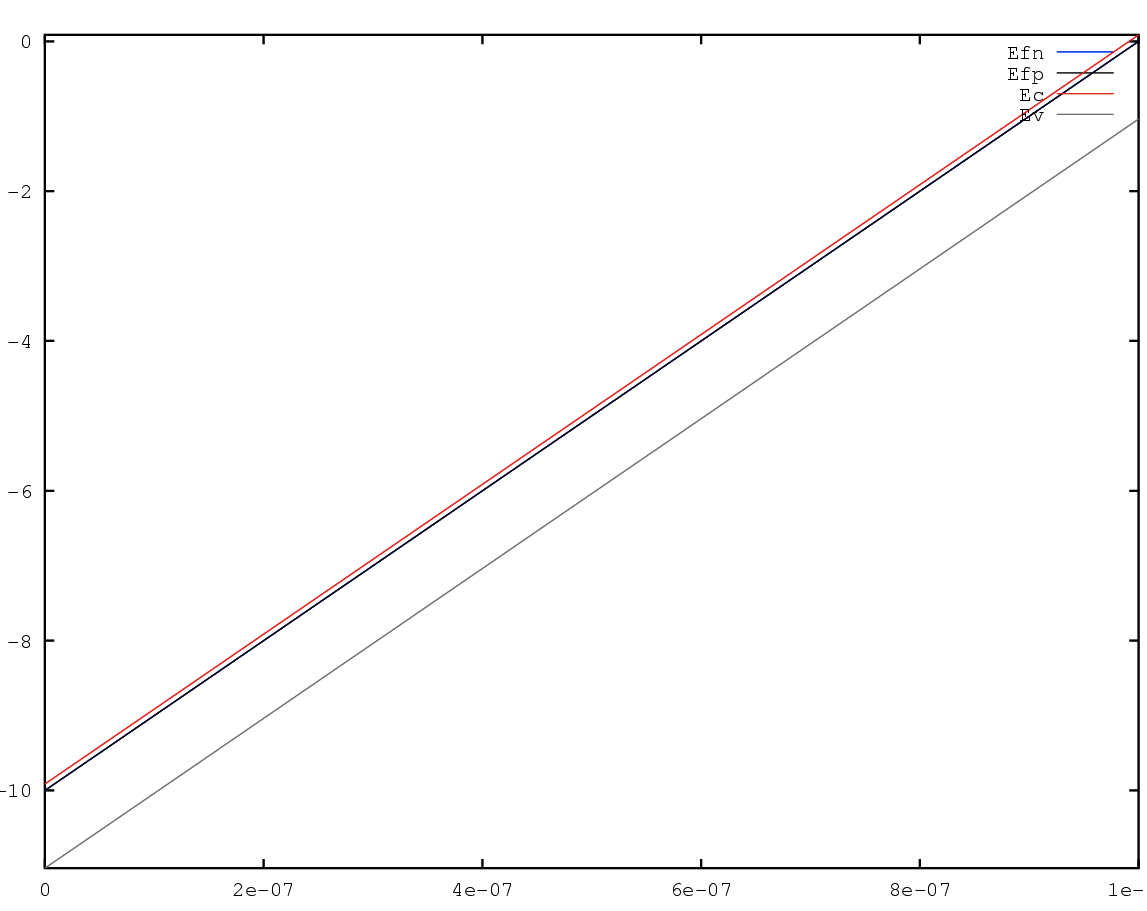
\includegraphics[width=.7\linewidth]{function/images/secs1d_dd_newton_819.png}
\caption{Figure produced by demo number 1 for function secs1d\_dd\_newton}
\label{fig:secs1d_dd_newton_figure_1}
\end{figure}
\clearpage
